\documentclass[11pt]{article}
\usepackage[english]{babel}
\usepackage[utf8]{inputenc}
\usepackage[T1]{fontenc}
\usepackage{float}
\usepackage{lmodern,amsmath,amssymb,amstext,amsfonts,mathrsfs,graphicx,caption, subcaption}
\usepackage[width=14cm]{geometry}
\usepackage[colorlinks,pdfpagelabels,pdfstartview = FitV,bookmarksnumbered = true, bookmarksopenlevel=section, linkcolor = black,hypertexnames = false,citecolor = black,pdfpagelabels=false]{hyperref}
\usepackage{tablefootnote}
%\usepackage{rotating}
\usepackage{textcmds, enumitem}
\usepackage{sidecap} %, indentfirst
\usepackage[labelfont={bf,sf},font={small},labelsep=space]{caption}
\usepackage{chngcntr} % 			** Damit die Bilder Tabellen und Gleichungen 
\counterwithin{figure}{section}	%	** alle nach Kapiteln nummeriert sind.
\counterwithin{table}{section}%		**
\counterwithin{equation}{section}%	**	

\begin{document}
	\section{Results}
	
	\subsection{Response Properties from symmetrical Recurrent Interaction Networks in Correlation with Feedforward Recurrent Alignment}
	
	The feedforward recurrent alignment, defined in the method under section \ref{sec:ffrec_definition} quantify the degree of how much the feedforward input is aligned with the direction that spanned the recurrent network. If the input is well aligned with the maximal eigenvector of the recurrent interaction $J$, the random noise in the response would be suppressed by the evoked response due to the selective amplification. That is, with response amplification
		\begin{equation} \label{eq:response_amplification}
			\mathbf{r}^* = \sum_{i = 1}^{n} \frac{(\mathbf{e}_i \cdot \mathbf{h}) \mathbf{e}_i}{1-\lambda_i} \, , 
		\end{equation}
	the steady state response is then dominated by the projection of the input vector $\mathbf{h}$ along the axis defined by the eigenvector $\mathbf{e}_{\text{max}}$ whose eigenvalue $\lambda_{\text{max}}$ is maximal and near one \cite{dayan2005theoretica}. 
		\begin{equation} \label{eq:selective_amplification}
			\mathbf{r}^* \approx \frac{(\mathbf{e}_{\text{max}} \cdot \mathbf{h}) \mathbf{e}_{\text{max}}}{1 - \lambda_{\text{max}}}
		\end{equation}
	The projection of input on eigenvector $\mathbf{e}_{\text{max}}$ reaches its maximal when $\mathbf{h}$ is approximately $\mathbf{e}_{\text{max}}$ itself. Therefore, the steady state responses reaches its maximum and the feedforward recurrent alignment equals the maximal eigenvalue $\lambda_{\text{max}}$ of $J$ because of (\ref{eq:ffrec_equals_eigval}). 
	
	On the other hand, if the input is not well aligned with the dominant eigenvectors, the random noise is large relative to the response. For an extreme example, if the input is aligned with the eigenvector with minimal eigenvalue $\lambda_{\text{min}}$, the response will almost not contribute to the steady state response at all due to the response amplification (\ref{eq:response_amplification}). This could also be reflected by the feedforward recurrent alignment, which equals $\lambda_{\text{min}}$ in this case because of (\ref{eq:ffrec_equals_eigval}). 
	
	We can thus conclude that the feedforward recurrent alignment (\ref{eq:ffrec_align}) reflects the alignment between the feedforward input and the dominant eigenvectors of the recurrent interaction network $J$. In the following sections, the four properties introduced at section \ref{sec:response_properties_for_evaluation} will be evaluated in the model and compare to the tendency observed in \cite{tragenap2023nature}. 
	
	\subsubsection{Trial-to-Trial Correlation increases with larger Alignment}
	
	As defined in the paragraph \ref{para:ttc_sym}, the inputs are constructed by multivariate normal distribution (\ref{eq:input_distribution}). To model the alignment of inputs with eigenvectors, the eigenvectors of the interaction matrix $J$ are chosen to be the the mean vector $\mathbf{\mu}$ for input distribution. That is
		\begin{equation}
			\mathbf{h_i} \sim \mathcal{N} (\mathbf{e}_i, \sigma_i^2\mathbf{I_n}) \, . 
		\end{equation}
	The degree of alignment of input on the dominant eigenvector $\mathbf{e}_{\text{max}}$ is then determined approximately by the size of eigenvalue, to which the eigenvector is corresponded. 
	
	%And as explained above, the better the input is aligned with the dominant eigenvector, the better the approximation. 
	
	We want to find out the correlation between the feedforward recurrent and the trial-to-trial correlation $\beta_s$, defined by (\ref{eq:ttc_sym}). Therefore, sort the eigenvectors in the order such that their corresponding eigenvalues are in ascending order. That is
		\begin{equation} \label{eq:ascending_order}
			\mathbf{e}_{\text{min}}, ..., \mathbf{e}_i, \mathbf{e}_j, ..., \mathbf{e}_{\text{max}} \, \, \text{such that} \, \, \lambda_{\text{min}} < ...< \lambda_i < \lambda_j < ... < \lambda_{\text{max}} \, ,
		\end{equation}
	with $\lambda_i$ the corresponding eigenvalue for eigenvector $\mathbf{e}_i$. As a result, the inputs that aligned with eigenvectors in this order have an increasing feeedforward recurrent alignment approximately. 
	
	Generating the results with (\ref{eq:steady_state_distribute}) for $N$ trials. The trial-to-trial correlation can be calculated with (\ref{eq:ttc_sym}). 
	\vspace{-0.4cm}
		\begin{SCfigure}[0.9][h] \label{fig:ttc_ffrec_sym}
			\centering
			\caption{\textbf{Correlation between feedforward recurrent alignment and trial to trial correlation.} Inputs aligned to eigenvectors $\mathbf{e}_i$ of interaction matrix $J$ in the ascending order of eigenvalues (\ref{eq:ascending_order}), resulting the feedforward recurrent alignment varies approximately between $\lambda_{\text{min}}$ and $\lambda_{\text{max}}$. For each input alignment to an eigenvector, $N$ trials of evoked responses were generated for calculation of the trial-to-trial correlation.}
			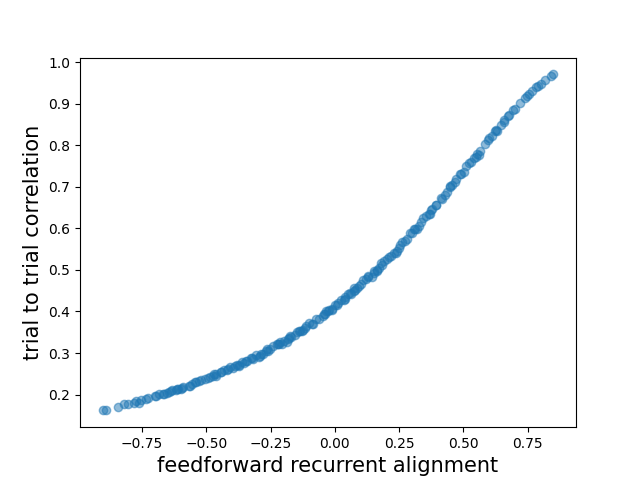
\includegraphics[width=0.5\textwidth]{../figures/ttc_sym.png}
		\end{SCfigure}
	
	We considered visually naive cortex as feedforward recurrent alignment equals zero, which could be interpreted as responses evoked by random inputs. The trial-to-trial correlation with random inputs is then smaller than the case, when the feedforward recurrent alignment takes the maximal value under inputs aligned with $\mathbf{e}_{\text{max}}$. This coincides with the experimental observations od responses from visually naive and experienced primary visual cortex of ferrets \cite{tragenap2023nature}. 
	
	Moreover, the modulation suggests a positive correlation between the feedforward recurrent alignment and the trial-to-trial correlation over the whole alignment range. The result confirms the idea that with the feedforward inputs more and more aligned with the dominant eigenvector of recurrent network, the stability between trials increases also simultaneously and almost continuously. The process of reaching higher trial-to-trial stability is therefore a process of becoming more aligned with the dominant eigenvector. 
	
	%The positive correlation between the feedforward recurrent alignment and the trial-to-trial correlation coincident with the experimental observations od responses from visually naive and experienced primary cortex of ferrets \cite{tragenap2023nature}. Moreover, the modulation suggests that 
	
	\subsubsection{Intra-Trial Stability increases with larger Alignment}
	
	Now we want to see if our modeling could capture the change in intra-trial stability during the development observed in the primary visual cortex of ferrets \cite{tragenap2023nature}. The intra-trial stability increased after the eye opening and a couple of days. The feedforward recurrent alignment hypothesis suggests that the visual experienced cortex should have a better alignment between feedforward inputs and the dominant modes in recurrent network. To confirm this idea, we would expect the intra-trial stability would be larger with better alignment between input and the dominant eigenvector. 
	
	Analogous to trial-to-trial correlation, the eigenvectors are sorted in the descending order according to the eigenvalues (\ref{eq:ascending_order}). The intra-trial stability is calculated with (\ref{eq:its_sym}).
	\vspace{-0.4cm}
	\begin{SCfigure}[0.9][h] 
		\centering
		\caption{\textbf{Correlation between feedforward recurrent alignment and intra-trial stability.} Inputs aligned to eigenvectors $\mathbf{e}_i$ of interaction matrix $J$ in the ascending order of eigenvalues (\ref{eq:ascending_order}), resulting the feedforward recurrent alignment varies approximately between $\lambda_{\text{min}}$ and $\lambda_{\text{max}}$. For each input alignment to an eigenvector, the intra-trial stability is calculated with the evoked steady state response.}
		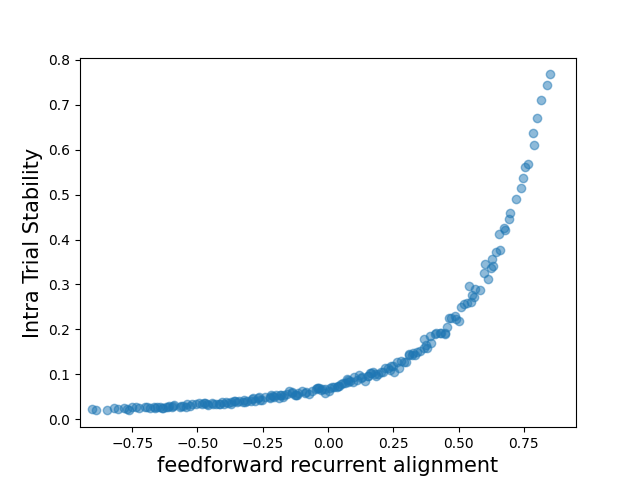
\includegraphics[width=0.5\textwidth]{../figures/its_sym.png}
		\label{fig:its_ffrec_sym}
	\end{SCfigure}

	The result (figure \ref{fig:its_ffrec_sym}) indicates also a positive correlation between the feedforward recurrent alignment and the intra-trial stability. With random feedforward inputs, the feedforward recurrent alignment take the value near zero. So the eye opening happens somewhere between feedforward recurrent equals zero and reaches maximal. Thus, before the eye opening, there is already certain alignment that lead to a certain degree of intra-trial correlation. 
	
	Furthermore, the correlation is almost exponential. So, the enhancement of the input alignment to the dominant eigenvector is more rapid after the eye opening than before the eye opening. One assumption for this phenomenon could be that after the eye opening, the environment provides more training data for the network so that the alignment between inputs and dominant eigenvector could be improved more efficiently. As a result, the responses get more intense and drive a better alignment forward. A positive loop could arise and speed up until the optimum is reached. 
	
	\subsubsection{Dimensionality decreases with larger Alignment}
	
	Dimensionality is a generally important property of neural representations and could help to understand processes for example in learning and controlling \cite{bartolo2020dimensionality, badre2021dimensionality}. A low dimensional representation will encode a diverse range of inputs into a small set of common, orthogonal activity patterns. In other words, low dimensional activity pattern require small number of basis vectors from the response space to represent itself. On the other hand, a high dimensional representation will separate even similar inputs into orthogonal activity patterns. Compare to low dimensional representation, a high dimensional activity pattern represents with a large set of basis vectors \cite{badre2021dimensionality}. 
	
	Therefore, we also aim to take a look at the change of dimensionality during the increase of alignment in the modeling. In ferrets primary visual cortex, the dimensionality decreased from days before eye opening to eye opening and then to days after eye opening \cite{tragenap2023nature}. We would then expect that the model should also suggest a decrease of dimensionality with increase of alignment between inputs and dominant eigenvector of recurrent network. 
	
	For a certain alignment, the principal component analysis reflects actually directly the dimensionality of the evoked activity pattern under this alignment. Because the principal components are the eigenvectors of response covariance, they also build up a set of basis vector for the activity pattern space. The variance ratio of principal components reflect the weight that each eigenvector takes to represent the activity pattern. Thus, if only a small number of principal components contributes the most, the activity pattern is then low dimensional. While if a broad set of principal components are similarly important, the activity pattern is high dimensional.  
	
	With the idea of earning the linear dimensionality defined as participation ratio based on the principal component analysis, the eigenvectors here are ordered in descending order, in the opposite order of ascending order defined above (\ref{eq:ascending_order}). That is 
		\begin{equation} \label{eq:descding_order}
			\mathbf{e}_{\text{max}}, ..., \mathbf{e}_i, \mathbf{e}_j, ..., \mathbf{e}_{\text{min}} \, \, \text{such that} \, \, \lambda_{\text{max}} > ...> \lambda_i > \lambda_j > ... > \lambda_{\text{min}} \, .
		\end{equation}
	%For the calculation of the linear dimensionality (\ref{eq:dim_analytical_sym}) and (\ref{eq:dim_empirical_sym}), 
	For the generation of inputs with covariance matrix $\mathbf{\Sigma^{\text{Dim}}}$ (\ref{eq:Sigma_dim}), a subset of eigenvectors $\{\mathbf{e}_i\}_{i = L, ..., L+M}$ will be chosen for $L=1, ..., \frac{n}{2}$. $M$ then determines how many eigenvectors will contribute to generate inputs and evoked activity. In each such subset of eigenvectors, the leading eigenvector is $\mathbf{e}_L$. Approximate here the feedforward recurrent alignment with the leading eigenvector only. Since $L$ is considered only in range of the first half of eigenvectors ordered as (\ref{eq:descding_order}), the range of feedforward recurrent alignment is between around $0$ and $\lambda_{\text{max}}$. The linear dimensionality analytically and empirically will be calculated according to (\ref{eq:dim_analytical_sym}) and (\ref{eq:dim_empirical_sym}). 
	
		\begin{figure}[H] 
			\centering
			\begin{subfigure}[b]{0.45\textwidth} 
				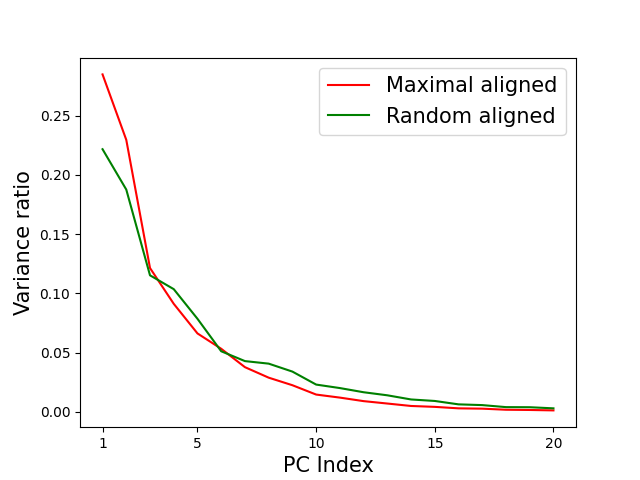
\includegraphics[width=\textwidth]{../figures/dim_align_rand_sym.png}
				\caption{}
			\end{subfigure}
			\begin{subfigure}[b]{0.45\textwidth}
				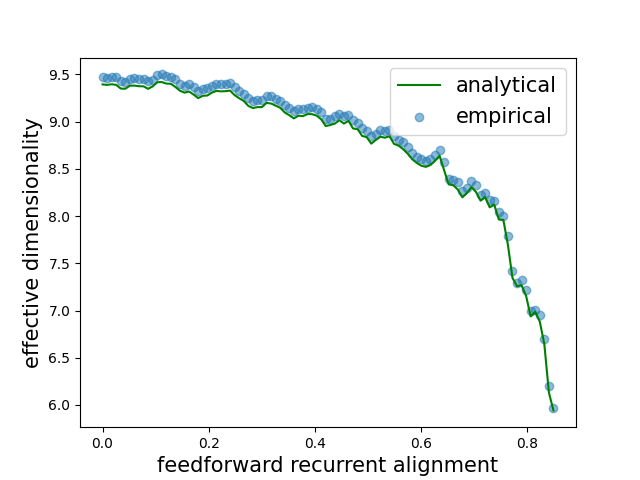
\includegraphics[width=\textwidth]{../figures/dim_sym.png}
				\caption{}
			\end{subfigure}
			\vspace{-0.2cm}
			\caption{\textbf{The correlation between dimensionality and feedforward recurrent alignment.} Prior experimental observation suggests that the dimensionality decreases from prior to post eye opening \cite{tragenap2023nature}. With the feedforward recurrent alignment hypothesis, dimensionality property of the neural representation could be captured. \textbf{(a)} Principal component analysis for the evoked activity under best alignment between inputs and dominant eigenvector and spontaneous random alignment. Red line for maximal alignment and green line for spontaneous alignment. \text{(b)} Achieve the correlation between dimensionality and feedforward recurrent alignment with analytical (\ref{eq:dim_analytical_sym}) and empirically (\ref{eq:dim_empirical_sym}). The green line displays the analytical approximation for dimensionality and the blue dots for empirical approximation.} 
			\label{fig:correlation_dim_ffrec_sym}
		\end{figure}
	\vspace{-0.2cm}
	As explained above, the principal component analysis helps to decode the dimensionality. The curve in figure \ref{fig:correlation_dim_ffrec_sym} (a) of the variance ratio reflects the dimensionality. Spontaneous random alignment has a flatter variance ratio curve, indicating a broader range of eigenvector contribution. Therefore, the spontaneous random alignment has a higher dimensionality. With the feedforward recurrent alignment hypothesis, the spontaneous random alignment matches the state before the eye opening and the maximal alignment for the state after eye opening. Therefore, the hypothesis results the same tendency of dimensionality decrease that observed in ferrets\cite{tragenap2023nature}.
	
	In total, a negative correlation between the dimensionality and feedforward recurrent alignment is shown in figure \ref{fig:correlation_dim_ffrec_sym} (b). The correlation forms nearly a flipped logarithmic function. The error between analytical and empirical results are small, which confirmed the well approximation formulated analytically by (\ref{eq:dim_analytical_sym}). 
	
	Besides, the flipped logarithmic correlation suggests the similar principle for intra-trial stability (figure \ref{fig:its_ffrec_sym}). After eye opening, the reduction of dimensionality becomes larger when the feedforward inputs aligns better with dominant eigenvector. It could be the case, that after the eye opening, the recurrent network tries to encode the environment information with large number of eigenvectors, which is costing for the system. After a period of time of getting used to the stimuli, the system speed up to find out a more efficient encoding with fewer eigenvectors and the information becomes more determined. 
	%After finding out a better solution, the improvement will be speed up until the optimum encoding with at least number of eigenvectors. 
	
	\subsubsection{Alignment to spontaneous activity increases with larger Alignment}
	
	Spontaneous activity in neural systems is defined as neural activity that is not driven by an external stimulus. The activity patterns of spontaneous activity is not completely random and have often unique spatiotemporal patterns that instruct neural circuit development in the developing brain. Moreover, normal and aberrant patterns of spontaneous activity underline behavioral states and diseased conditions in adult brains. Therefore, the spontaneous activity is essential for the understanding of brain development \cite{imaizumi2018spontaneous}. The alignment between activity pattern and spontaneous activity pattern could show the structural relation between patterns. Besides, it could also reflect the presentation of spontaneous activity in other activity patterns. 
	
	In baby ferrets' brain, a transformation from visual responses that are loosely aligned with spontaneous activity in the cortex before eye opening to the reliable and well aligned responses several days after eye opening were observed \cite{tragenap2023nature}. Thus, we will expect that the feedforward recurrent hypothesis can reflect the tendency that evoked activity aligned better to spontaneous activity during the development of brain. 
	\vspace{-0.4cm}
		\begin{figure}[H] 
			\centering
			\begin{subfigure}[b]{0.45\textwidth} 
				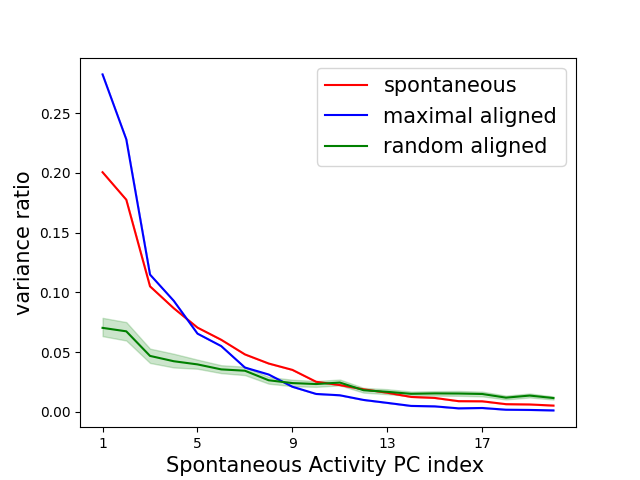
\includegraphics[width=\textwidth]{../figures/align_to_spont_act_variance_ratio.png}
				\caption{}
			\end{subfigure}
			\begin{subfigure}[b]{0.45\textwidth}
				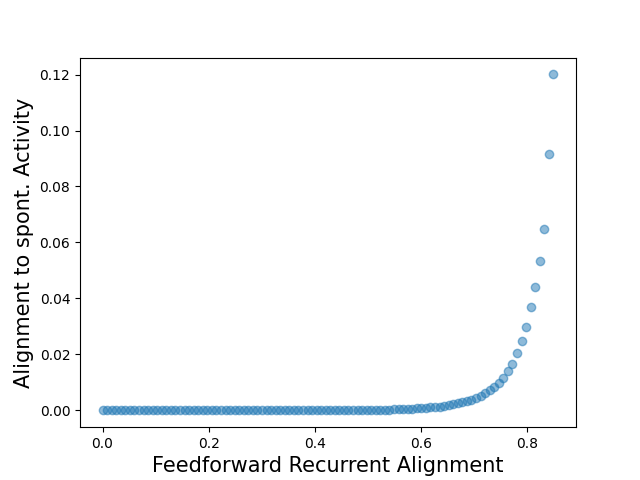
\includegraphics[width=\textwidth]{../figures/spont_align_ffrec_sym.png}
				\caption{}
			\end{subfigure}
			%\vspace{-0.1cm}
			\caption{\textbf{Correlation between alignment to spontaneous activity and feedforward recurrent alignment.} Spontaneous activity reflects inputs from wide range of different sources and considered to already aligned to the recurrent network\cite{tragenap2023nature}. Aligning activity patterns to spontaneous activity is in principle to explain the activity pattern by the principal components of spontaneous activity. \textbf{(a)} Variance ratio (\ref{eq:var_explain_spont_act_sym}) of spontaneous activity, evoked activity by feedforward input maximally aligning to recurrent network, and evoked activity by randomly aligning to recurrent network explained by principal components of spontaneous activity. The red line illustrates the variance ratio of spontaneous activity, blue line the maximal alignment, and green line the random alignment. Shadow shows the 95\% confident interval for 50 networks. \text{(b)} The correlation between final alignment score to spontaneous activity and feedforward recurrent alignment better than random alignment calculated with (\ref{eq:align_to_spont_act_sym}). The eigenvalues are ordered in the same way as (\ref{eq:descding_order}). Only the first half eigenvectors are taken into account to determine the correlation.}
			\label{fig:align_spont_act_sym}
		\end{figure}
	
	Under the assumption that at eye opening, the patterns of feedforward inputs are not as well aligned to the recurrent network as the spontaneous activity, the evoked and spontaneous pattern overlaps only little (figure \ref{fig:align_spont_act_sym}(a), visually comparing green line to red line.) It could be observed here that only the last few principal components has the similar variance ratio, while the first few dominant eigenvectors differs a lot. On the contrary, experience-driven changes that optimize the feedforward-recurrent alignment results in a stronger overlap between distributions of evoked and spontaneous activity pattern (figure \ref{fig:align_spont_act_sym}(a), visually comparing red line to blue line.). Most of the principal components has the similar explained variance ratio. In both cases, the hypothesis matches experimental observations in baby ferrets' brain \cite{tragenap2023nature}.
	
	To visualize and quantify the overlap between activity patterns from evoked and endogenous pattern, we considered the summarized alignment score (\ref{fig:align_spont_act_sym}). A exponential correlation between alignment to spontaneous activity and feedforward recurrent alignment (figure \ref{fig:align_spont_act_sym}(b)) is suggested by the modeling. The strong growth of overlaps between evoked and endogenous activity starts only shortly before the optimal experience-driven alignment, indicating that the alignment could require a large amount of experience and training. The costly process to optimal alignment to spontaneous activity could on the other hand reflect the importance of the connection between evoked and endogenous activity patterns. 

	
\end{document}